%----------------------------------------------------------
% Capítulo 3 – Desarrollo
%----------------------------------------------------------

%----------------------------------------------------------
\section{Base de datos}
%----------------------------------------------------------

\begin{large}

Para esta plataforma, la base de datos se implementó íntegramente en Firestore, aprovechando su modelo NoSQL en tiempo real y su escalabilidad automática. A continuación se describen los pasos clave:

\end{large}

\subsection{Configuración inicial en Firebase}

\begin{large}

En primer lugar, se creó un proyecto en la consola de Firebase y se habilitaron los servicios de Firestore y Authentication. Dentro de Firestore, se generó la colección raíz \textit{businesses}, donde cada documento tiene un identificador único (\textit{businessId}). De forma automática, Firestore asigna una referencia a cada colección y subcolección cuando se insertan documentos por primera vez desde los clientes.

Para conectar la aplicación iOS, se descargó el archivo \textit{GoogleService-Info.plist} desde la consola de Firebase y se añadió al directorio principal del proyecto Xcode. En el caso del portal web, se obtuvo el objeto de configuración (API key, project ID, etc.), se guardó en un archivo \textit{.env} y se cargó desde un archivo \textit{config.ts} bajo \textit{/src/firebase}.

\end{large}

\subsection{Modelo de datos en Firestore}

\begin{large}

\begin{lstlisting}[language={},basicstyle=\ttfamily\small, caption={Modelo de datos en Firestore}]
/businesses/{businessId}
    |-- name
    |-- tagline (nullable)
    |-- address
    |-- city
    |-- country
    |-- postcode
    |-- taxId (CIF in Spain, VAT in the UK, EIN in the USA, etc.)
    |-- email
    |-- phone
    |-- createdAt
    |-- subscriptionPlan: "free" | "premium"
    |-- storageLimit: "1 month" | "unlimited"
    |
    |-- employees/{employeeId}
    |        |-- userId (linked to Firebase Auth)
    |        |-- name
    |        |-- email (linked to Firebase Auth)
    |        |-- phone
    |        |-- role: "admin" | "employee" (linked to Firebase Auth)
    |        |-- joinedAt
    |
    |-- clients/{clientId}
    |        |-- userClientId (linked to Firebase Auth) ??
    |        |-- companyName
    |        |-- clientName
    |        |-- address
    |        |-- city
    |        |-- country
    |        |-- postcode
    |        |-- email (linked to Firebase Auth)
    |        |-- phone
    |        |-- createdAt
    |
    |-- invoices/{invoiceId}
    |        |-- issuedAt
    |        |-- dueDate
    |        |-- status: "Paid" | "Pending" | "Overdue"
    |        |-- subtotal
    |        |-- taxTotal
    |        |-- discounts
    |        |-- totalAmount
    |        |-- currency
    |        |-- clientId
    |        |-- employeeId
    |        |-- pdfURL (Cloudflare)
    |        |-- deleteAfter (Free plan: issuedAt + 1 month,
                                Premium plan: unlimited)
    |        |-- productsStack/{productStackId}
    |                          |-- productId
    |                          |-- supplyDate
    |                          |-- quantity
    |                          |-- amount
    |                          |-- taxRate
    |                          |-- taxNet
    |
    |-- products/{productId}
    |        |-- description
    |        |-- unitPrice
\end{lstlisting}

\begin{description}[leftmargin=3cm, style=nextline]
  \item[\textit{businesses/\{businessId\}}] Documento principal que contiene datos generales de la empresa (nombre, contactos, identificación fiscal, suscripción y límites de almacenamiento) y agrupa subcolecciones.
  \item[\textit{businesses/\{businessId\}/employees/\{employeeId\}}] Empleados de la empresa, con referencia a Firebase Auth, datos de contacto y rol.
  \item[\textit{businesses/\{businessId\}/clients/\{clientId\}}] Clientes asociados a la empresa, con datos de contacto y posible vinculación a Firebase Auth.
  \item[\textit{businesses/\{businessId\}/invoices/\{invoiceId\}}] Facturas emitidas por la empresa, con fechas, estado, importes y subcolección \textit{productsStack} para desglosar cada línea de producto (ID de producto, cantidad, impuesto, etc.).
  \item[\textit{businesses/\{businessId\}/products/\{productId\}}] Productos que la empresa ofrece, con descripción y precio unitario.
\end{description}

Esta organización centraliza la lógica de datos y asegura coherencia en todos los clientes, facilitando la mantenibilidad y escalabilidad del sistema.

\end{large}

\subsection{Reglas de seguridad de Firestore}

\begin{large}

Para garantizar que solo los usuarios autorizados accedieran a la información, se definieron reglas en el panel de Firestore. Un extracto de las reglas más relevantes es:

\begin{lstlisting}[language={}, caption={Reglas de seguridad de Firestore}]
rules_version = '2';
service cloud.firestore {
  match /databases/{database}/documents {
    
    // Raiz de negocios: controlamos creacion/lectura/actualizacion/borrado a nivel de negocio
    match /businesses/{businessId} {
      // Cualquiera autenticado puede leer la informacion de un negocio
      allow read: if request.auth != null;
      // Cualquiera autenticado puede crear un nuevo negocio
      allow create: if request.auth != null;
      // Solo un admin (claim role == "admin") puede modificar o borrar un negocio
      allow update, delete: if request.auth.token.role == 'admin';
      
      // Subcoleccion de empleados: solo admins pueden gestionar empleados
      match /employees/{employeeId} {
        allow read: if request.auth != null;
        allow create, update, delete: if request.auth.token.role == 'admin';
      }
      
      // Subcoleccion de clientes: 
      //   - cualquiera autenticado ve datos de clientes
      //   - un admin o el propio cliente (uid == userClientId) puede crear/editar/borrar
      match /clients/{clientId} {
        allow read: if request.auth != null;
        allow create: if request.auth.token.role == 'admin';
        allow update, delete: if request.auth.token.role == 'admin'
                              || request.auth.uid == resource.data.userClientId;
      }
      
      // Subcoleccion de facturas:
      //   - cualquiera autenticado puede leer
      //   - crear: admin o empleado que firma la factura (employeeId en request.resource.data)
      //   - actualizar: admin o empleado que creo la factura (employeeId en el dato existente)
      //   - borrar: solo admin
      match /invoices/{invoiceId} {
        allow read: if request.auth != null;
        allow create: if request.auth.token.role == 'admin'
                      || request.auth.uid == request.resource.data.employeeId;
        allow update: if request.auth.token.role == 'admin'
                      || request.auth.uid == resource.data.employeeId;
        allow delete: if request.auth.token.role == 'admin';
        
        // Dentro de cada factura, la subcoleccion de lineas de producto:
        //   - cualquiera autenticado puede leer
        //   - solo el admin puede escribir/borrar
        match /productsStack/{productStackId} {
          allow read: if request.auth != null;
          allow create, update, delete: if request.auth.token.role == 'admin';
        }
      }
      
      // Subcoleccion de productos: 
      //   - cualquiera autenticado puede leer
      //   - solo admin puede escribir/borrar
      match /products/{productId} {
        allow read: if request.auth != null;
        allow create, update, delete: if request.auth.token.role == 'admin';
      }
    }
    
  }
}
\end{lstlisting}

Con estas reglas, solo el administrador (rol \textit{admin}) puede crear o eliminar facturas y productos, y cada empleado (rol \textit{employee}) puede crear o actualizar facturas que él mismo genere. Los clientes solo acceden a sus propios documentos, y todas las operaciones requieren un usuario autenticado (\textit{request.auth != null}), lo que cumple con los requisitos de seguridad y protección de datos.

\end{large}

%----------------------------------------------------------
\section{Implementación iOS}
%----------------------------------------------------------

\begin{large}

En esta sección profundizamos en la aplicación iOS, donde se dedicaron la mayoría de las horas de desarrollo. Partimos desde cero, aprendiendo Swift y SwiftUI, y construimos la app siguiendo el patrón MVVM para separar responsabilidades y lograr un código más mantenible.

\end{large}

\subsection{Configuración del proyecto y conexión a Firebase}

\begin{large}

Para iniciar el proyecto, se utilizó Xcode 16.3 con la plantilla de SwiftUI. Los pasos fueron:

\begin{enumerate}
  \item En Xcode, crear un nuevo proyecto seleccionando \emph{App} y, como lenguaje, \textbf{Swift} con interfaz \textbf{SwiftUI}.
  \item Descargar \textit{GoogleService-Info.plist} desde la consola de Firebase y arrastrarlo al grupo raíz del proyecto en Xcode. Asegurarse de marcar la opción de agregarlo a todos los targets.
  \item Instalar el paquete oficial de Firebase mediante Swift Package Manager (\emph{File → Add Packages…}), usando la URL \url{https://github.com/firebase/firebase-ios-sdk.git}.
  \item En el archivo \textit{QuickBillApp.swift}, inicializar Firebase antes de cargar la escena principal:
    \begin{lstlisting}[language={swift}, caption={Inicialización de Firebase en QuickBillApp.swift}]
    import SwiftUI
    import FirebaseCore
    
    @main
    struct QuickBillApp: App {
        @StateObject private var auth = AuthViewModel()
        @AppStorage("appLanguage") private var appLanguage: String = AppLanguage.english.rawValue
        
        init() {
            FirebaseApp.configure()
        }
        
        var body: some Scene {
            WindowGroup {
                if auth.isSignedIn {
                    MainTabView()
                } else {
                    StartView()
                }
            }
            .environmentObject(auth)
            .environment(\.locale, Locale(identifier: appLanguage))
        }
    }
    \end{lstlisting}
  \item Configurar en la consola de Firebase el dominio de la app, activando Authentication con correo/contraseña.
\end{enumerate}

Con estos pasos, la aplicación iOS ya está conectada a Firebase y lista para consumir Firestore y Authentication.

\end{large}

\subsection{Arquitectura MVVM}

\begin{large}

La aplicación iOS se organiza siguiendo el patrón \textit{Model–View–ViewModel} (MVVM). En la Figura~\ref{fig:models_folder} se muestra la distribución real de carpetas dentro de Xcode, enfocándose en la carpeta de los modelos:

\begin{figure}[H]
\centering
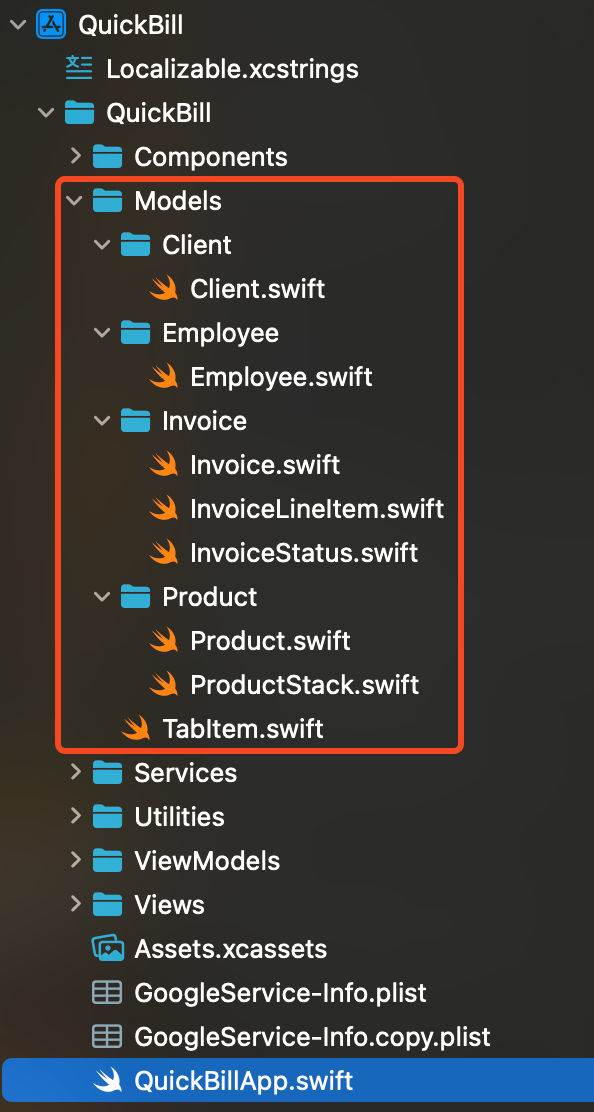
\includegraphics[width=0.5\textwidth]{Ilustraciones/ios_models_folder.png}
\caption{Estructura de la carpeta \textit{Models} en Xcode}
\label{fig:models_folder}
\end{figure}

A continuación se describe brevemente el propósito de cada grupo.

\textit{Models} agrupa todas las entidades que reflejan los documentos de Firestore. Cada subcarpeta contiene un único fichero con la estructura correspondiente:
\begin{itemize}
  \item \textbf{Client/Client.swift}: define la estructura \textit{Client} con campos básicos de la empresa o persona a facturar.
  \item \textbf{Employee/Employee.swift}: representa a cada empleado que accede a la app. Incluye su \textit{userId} (Firebase Auth), nombre, email, teléfono y rol.
  \item \textbf{Invoice}:
    \begin{itemize}
      \item \textit{Invoice.swift}: entidad principal con fechas, importes y referencias a cliente y empleado.
      \item \textit{InvoiceLineItem.swift}: describe cada línea de producto/servicio dentro de una factura.
      \item \textit{InvoiceStatus.swift}: \textit{enum} con los estados \textit{paid}, \textit{pending} y \textit{overdue}.
    \end{itemize}
  \item \textbf{Product}:
    \begin{itemize}
      \item \textit{Product.swift}: catálogo de productos con descripción y precio unitario.
      \item \textit{ProductStack.swift}: colección de productos que se añaden a una factura.
    \end{itemize}
  \item \textit{TabItem.swift}: enumeración con los tabs de navegación de la app.
\end{itemize}

\textit{Services} agrupa la lógica que no depende de la UI pero tampoco encaja como modelo puro:
\begin{itemize}
  \item \textit{AuthService.swift}: envoltorio sencillo sobre Firebase Auth con la finalidad de persistir la sesión de los usuarios en la aplicación.
  \item \textit{InvoicePDFBuilder.swift}: genera el PDF de una factura usando UIGraphicsPDFRenderer; recibe una instancia \textit{Invoice} y devuelve la URL local del fichero.
  \item \textit{InvoiceStatusService.swift}: actualiza el estado de una factura (\textit{paid}, \textit{pending}, \textit{overdue}) según \textit{issuedAt}, \textit{dueDate} y el \textit{status} almacenado.
\end{itemize}

\textit{Utilities} contiene código de soporte reutilizable. Actualmente sólo incluye \textit{AppLanguage.swift}, una enumeración para cambiar el idioma de la interfaz mediante la propiedad \textit{@AppStorage('appLanguage')}.

\textit{ViewModels} se divide en subcarpetas por dominio de negocio:
\begin{itemize}
  \item \textbf{Authentication}: gestiona el inicio de sesión, registro y la opción de 'ovidé mi contraseña'.
  \item \textbf{Clients}: gestión de listado, creación, borrado y edición de clientes.
  \item \textbf{Invoice}: \textit{InvoiceListViewModel.swift}, \textit{InvoiceDetailViewModel.swift} y \textit{AddInvoiceViewModel.swift} para listar, mostrar los detalles y crear nuevas faturas.
  \item \textbf{Products}: ViewModel para el catálogo de productos.
  \item \textbf{Settings}: controla las preferencias de la app.
  \item Además, en la raíz de la carpeta está \textit{AuthViewModel.swift}, que mantiene el estado global de autenticación y se inyecta como \textit{EnvironmentObject}.
\end{itemize}

\textit{Views} organiza las pantallas SwiftUI con la misma lógica de dominios:
\begin{itemize}
  \item \textbf{Authentication}: vistas de inicio de sesión y registro.
  \item \textbf{Clients}: lista de clientes y formulario de creación y edición.
  \item \textbf{Home}: vista inicial tras iniciar sesión (dashboard con todas las facturas).
  \item \textbf{Invoice}: formulario de creación y detalles de las facturas.
  \item \textbf{Products}: listado y formulario de productos.
  \item \textbf{Settings}: ajustes de idioma y cuenta.
  \item \textit{MainTabView.swift}: barra de pestañas inferior que enlaza \textit{Home}, \textit{Products}, \textit{Invoice}, \textit{Clients}, y \textit{Settings}.
  \item \textit{StartView.swift}: pantalla que decide si mostrar la vista de autenticación o el \textit{MainTabView} según el estado de \textit{AuthViewModel}.
\end{itemize}

Esta distribución favorece la separación de responsabilidades, donde los 
ViewModels actúan como enlace entre modelos y vistas, y cada conjunto de vistas se mantiene cohesionado dentro de su propio dominio y los modelos definen la estructura de los datos que se manejan.

\end{large}

\subsection{Generación de PDF}

\begin{large}

En lugar de recurrir a Cloud Functions, la app genera el PDF de la factura localmente a través del servicio \textit{InvoicePDFBuilder}. El proceso se resume a continuación; el código completo puede consultarse en el repositorio público.

\begin{enumerate}
  \item \textbf{Crear el lienzo A4}\newline
  Se instancia un \textit{UIGraphicsPDFRenderer} con tamaño A4 y metadatos del documento:
  \begin{lstlisting}[language=swift, basicstyle=\ttfamily\small, caption={Creación del lienzo A4}]
let bounds = CGRect(x: 0, y: 0, width: 595, height: 842) // A4 @72 dpi
let format = UIGraphicsPDFRendererFormat()
format.documentInfo = [
  kCGPDFContextCreator: "QuickBill",
  kCGPDFContextAuthor : "QuickBill"
]
let renderer = UIGraphicsPDFRenderer(bounds: bounds, format: format)
  \end{lstlisting}

  \item \textbf{Dibujar encabezados}\newline
  Dentro del bloque \textit{renderer.pdfData \{ ctx in …\}}, se escribe el título y los datos de empresa y cliente:
  \begin{lstlisting}[language=swift, basicstyle=\ttfamily\small, caption={Dibujar encabezados}]
ctx.beginPage()
"INVOICE".draw(at: CGPoint(x: bounds.midX-40, y:36),
               withAttributes: titleAttr)

drawBlock(label: "Your company", lines: [businessName])
drawBlock(label: "Bill to", lines: [clientName])
  \end{lstlisting}

  \item \textbf{Renderizar la tabla de productos}\newline
  Se imprime la cabecera y, para cada elemento de \textit{products}, se dibujan descripción, cantidad, precio unitario y total.

  \item \textbf{Calcular importes}\newline
  Al final se muestran subtotal, impuestos, descuentos y el TOTAL resaltado:
  \begin{lstlisting}[language=swift, basicstyle=\ttfamily\small, caption={Calcular importes}]
amountRow("Subtotal",  invoice.subtotal)
amountRow("Tax",       invoice.taxTotal)
amountRow("Discounts", invoice.discounts)
amountRow("TOTAL",     invoice.totalAmount, bold: true)
  \end{lstlisting}

  \item \textbf{Guardar en \textit{Documents}}\newline
  El PDF resultante se escribe como \textit{Invoice-<id>.pdf} en el sandbox de la app y se devuelve la URL para compartir o previsualizar.
\end{enumerate}

Este enfoque permite al usuario generar la factura al instante, sin incurrir en costes adicionales. Para la numeración se reutiliza el \textit{invoice.id} otorgado por Firestore, garantizando unicidad sin contadores globales.

\medskip
\noindent\textit{Código completo:} \url{https://github.com/JuanCarlosAcostaPeraba/QuickBill-App/blob/main/iOS/QuickBill/Services/InvoicePDFBuilder.swift}

\end{large}

\subsection{Autenticación y permisos}

\begin{large}

La autenticación se resuelve con Firebase Auth usando correo y contraseña. La lógica de inicio de sesión se  encapsula en el \textit{SignInViewModel}, mientras que la interfaz se construye en \textit{SignInView}. A grandes rasgos:

\begin{itemize}
  \item \textbf{SignInViewModel.swift}
    \begin{itemize}
      \item Propiedades \textit{@Published} para \textit{email}, \textit{password}, estado de alerta y bandera \textit{didSignIn}.
      \item Método \textit{signIn()} que llama a \textit{Auth.auth().signIn(withEmail:password:)} dentro de una \textit{Task}\,/\textit{await} y gestiona los posibles errores.
    \end{itemize}
  \item \textbf{SignInView.swift}
    \begin{itemize}
      \item Campos \textit{TextField} y \textit{SecureField} enlazados al ViewModel.
      \item Botón “Sign in” que ejecuta \textit{await viewModel.signIn()}; si la autenticación tiene éxito se activa \textit{auth.isSignedIn = true} (estado global mediante \textit{AuthViewModel}).
      \item Enlace a la vista de registro y a la de “Forgot password”.
    \end{itemize}
\end{itemize}

\noindent\textbf{Fragmento clave de autenticación:}
\begin{lstlisting}[language=swift, basicstyle=\ttfamily\small, caption={SignInViewModel.signIn()}]
@MainActor
func signIn() async {
    do {
        _ = try await Auth.auth()
            .signIn(withEmail: email, password: password)
        didSignIn = true
    } catch {
        alertMessage = error.localizedDescription
        showAlert = true
    }
}
\end{lstlisting}

\noindent Una vez autenticado, el UID se usa para filtrar datos, por ejemplo:

\begin{lstlisting}[language=swift, basicstyle=\ttfamily\small, caption={Filtrado de facturas por empleado}]
let uid = Auth.auth().currentUser?.uid ?? ""
Firestore.firestore()
  .collection("businesses")
  .document(businessId)
  .collection("invoices")
  .whereField("employeeId", isEqualTo: uid)
  .getDocuments { snapshot, error in ... }
\end{lstlisting}

El código completo de la pantalla de inicio de sesión, así como del \textit{SignInViewModel}, puede consultarse en GitHub:
\url{https://github.com/JuanCarlosAcostaPeraba/QuickBill-App/tree/main/iOS/QuickBill/Views/Authentication}

\end{large}

\subsection{Filtrado avanzado}

\begin{large}

Para mejorar la usabilidad, se implementó un sistema de filtrado avanzado en la lista de facturas. El usuario puede filtrar por cliente, estado, rango de fechas y rango de importe. Esta funcionalidad se encuentra en \textit{HomeView} y se gestiona a través del \textit{InvoiceListViewModel}.

\begin{lstlisting}[language=swift, basicstyle=\ttfamily\small, caption={HomeView.swift - Filtrado avanzado}]
var filteredInvoices: [Invoice] {
    invoices.filter { inv in
        (selectedStatus == .all || inv.status == selectedStatus) &&
        (
            searchText.isEmpty ||
            inv.companyName.lowercased().contains(searchText.lowercased()) ||
            dateFormatter.string(from: inv.issuedAt).contains(searchText) ||
            String(format: "%.2f", inv.totalAmount).contains(searchText)
        ) && (
            !enableDateFilter ||
            (
                (dateFrom == nil || inv.issuedAt >= dateFrom!) &&
                (dateTo   == nil || inv.issuedAt <= dateTo!)
            )
        ) && (
            !enableAmountFilter ||
            (
                (minTotal == nil || inv.totalAmount >= minTotal!) &&
                (maxTotal == nil || inv.totalAmount <= maxTotal!)
            )
        ) &&
        (selectedClientId == nil || inv.clientId == selectedClientId)
    }
}
\end{lstlisting}

El usuario puede seleccionar el estado de la factura, introducir texto para buscar por cliente o fecha, y activar los filtros de fecha e importe. El resultado se actualiza dinámicamente en la vista.

\end{large}

\subsection{UI/UX y pruebas en simulador}

\begin{large}

La interfaz de usuario se diseñó siguiendo las pautas de Apple para SwiftUI, priorizando la simplicidad y la usabilidad. Se utilizaron componentes estándar como \textit{List}, \textit{Form}, \textit{NavigationView} y \textit{Button} para construir una experiencia coherente.

Se priorizó la accesibilidad y la claridad visual mediante la asignación de colores distintivos a los diferentes estados de las facturas (verde para \textit{paid}, lila para \textit{pending} y rojo para \textit{overdue}), así como la incorporación de animaciones suaves en las transiciones de pantalla. Para la visualización de productos, se optó por \textit{LazyVGrid}, lo que permite una disposición adaptable y eficiente en distintos tamaños de pantalla.

Para verificar que todo funciona, se realizaron pruebas manuales en el simulador de iOS:

\begin{itemize}
  \item Crear una nueva factura: abrir \textit{AddInvoiceView}, rellenar campos, pulsar “Guardar” y comprobar que aparece en \textit{HomeView}.
  \item Editar estado de factura: marcar una factura pendiente como “Paid” y verificar que cambia su color (verde) en la lista.
  \item Generar PDF: pulsar “Generar PDF” en \textit{InvoiceDetailView} y verificar que se guarda en la carpeta \emph{Documents} del simulador.
  \item Inicio de sesión: probar con credenciales correctas e incorrectas para validar la lógica de \textit{Auth}.
\end{itemize}

A continuación se muestran algunas capturas de pantalla que ilustran estos flujos.

\begin{figure}[H]
  \centering
  %------------- Fila 1 -------------
  \begin{minipage}[t]{0.45\textwidth}
    \centering
    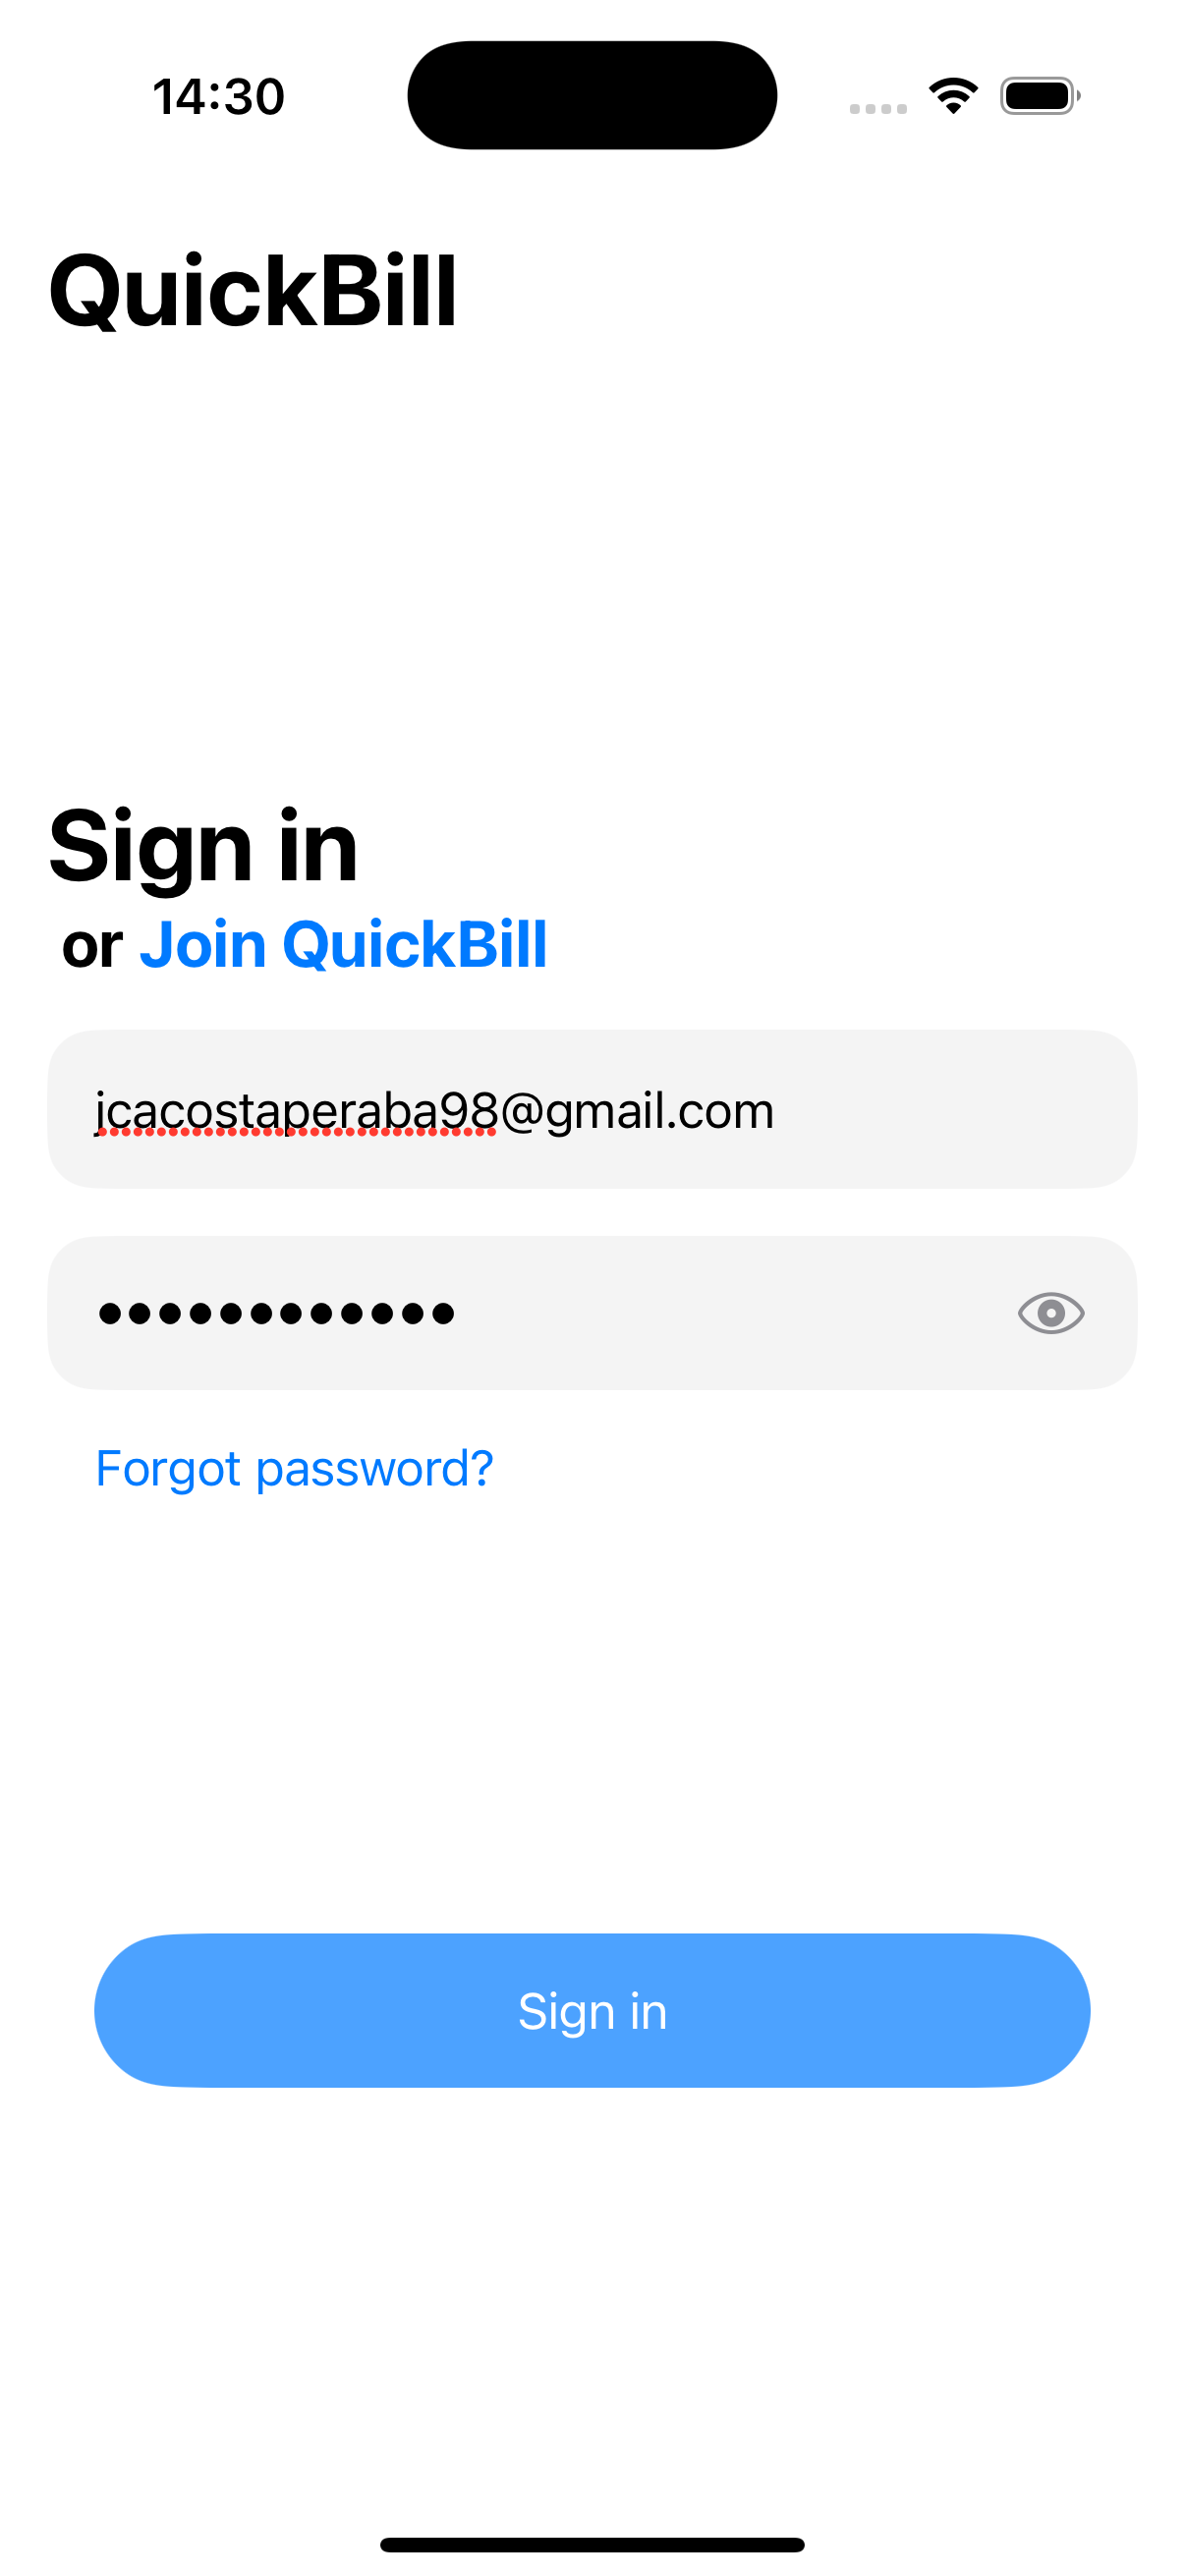
\includegraphics[width=0.8\textwidth]{Ilustraciones/ios_sign_in.png}
    \caption{Pantalla de inicio de sesión}
    \label{fig:ios_sign_in}
  \end{minipage}\hfill
  \begin{minipage}[t]{0.45\textwidth}
    \centering
    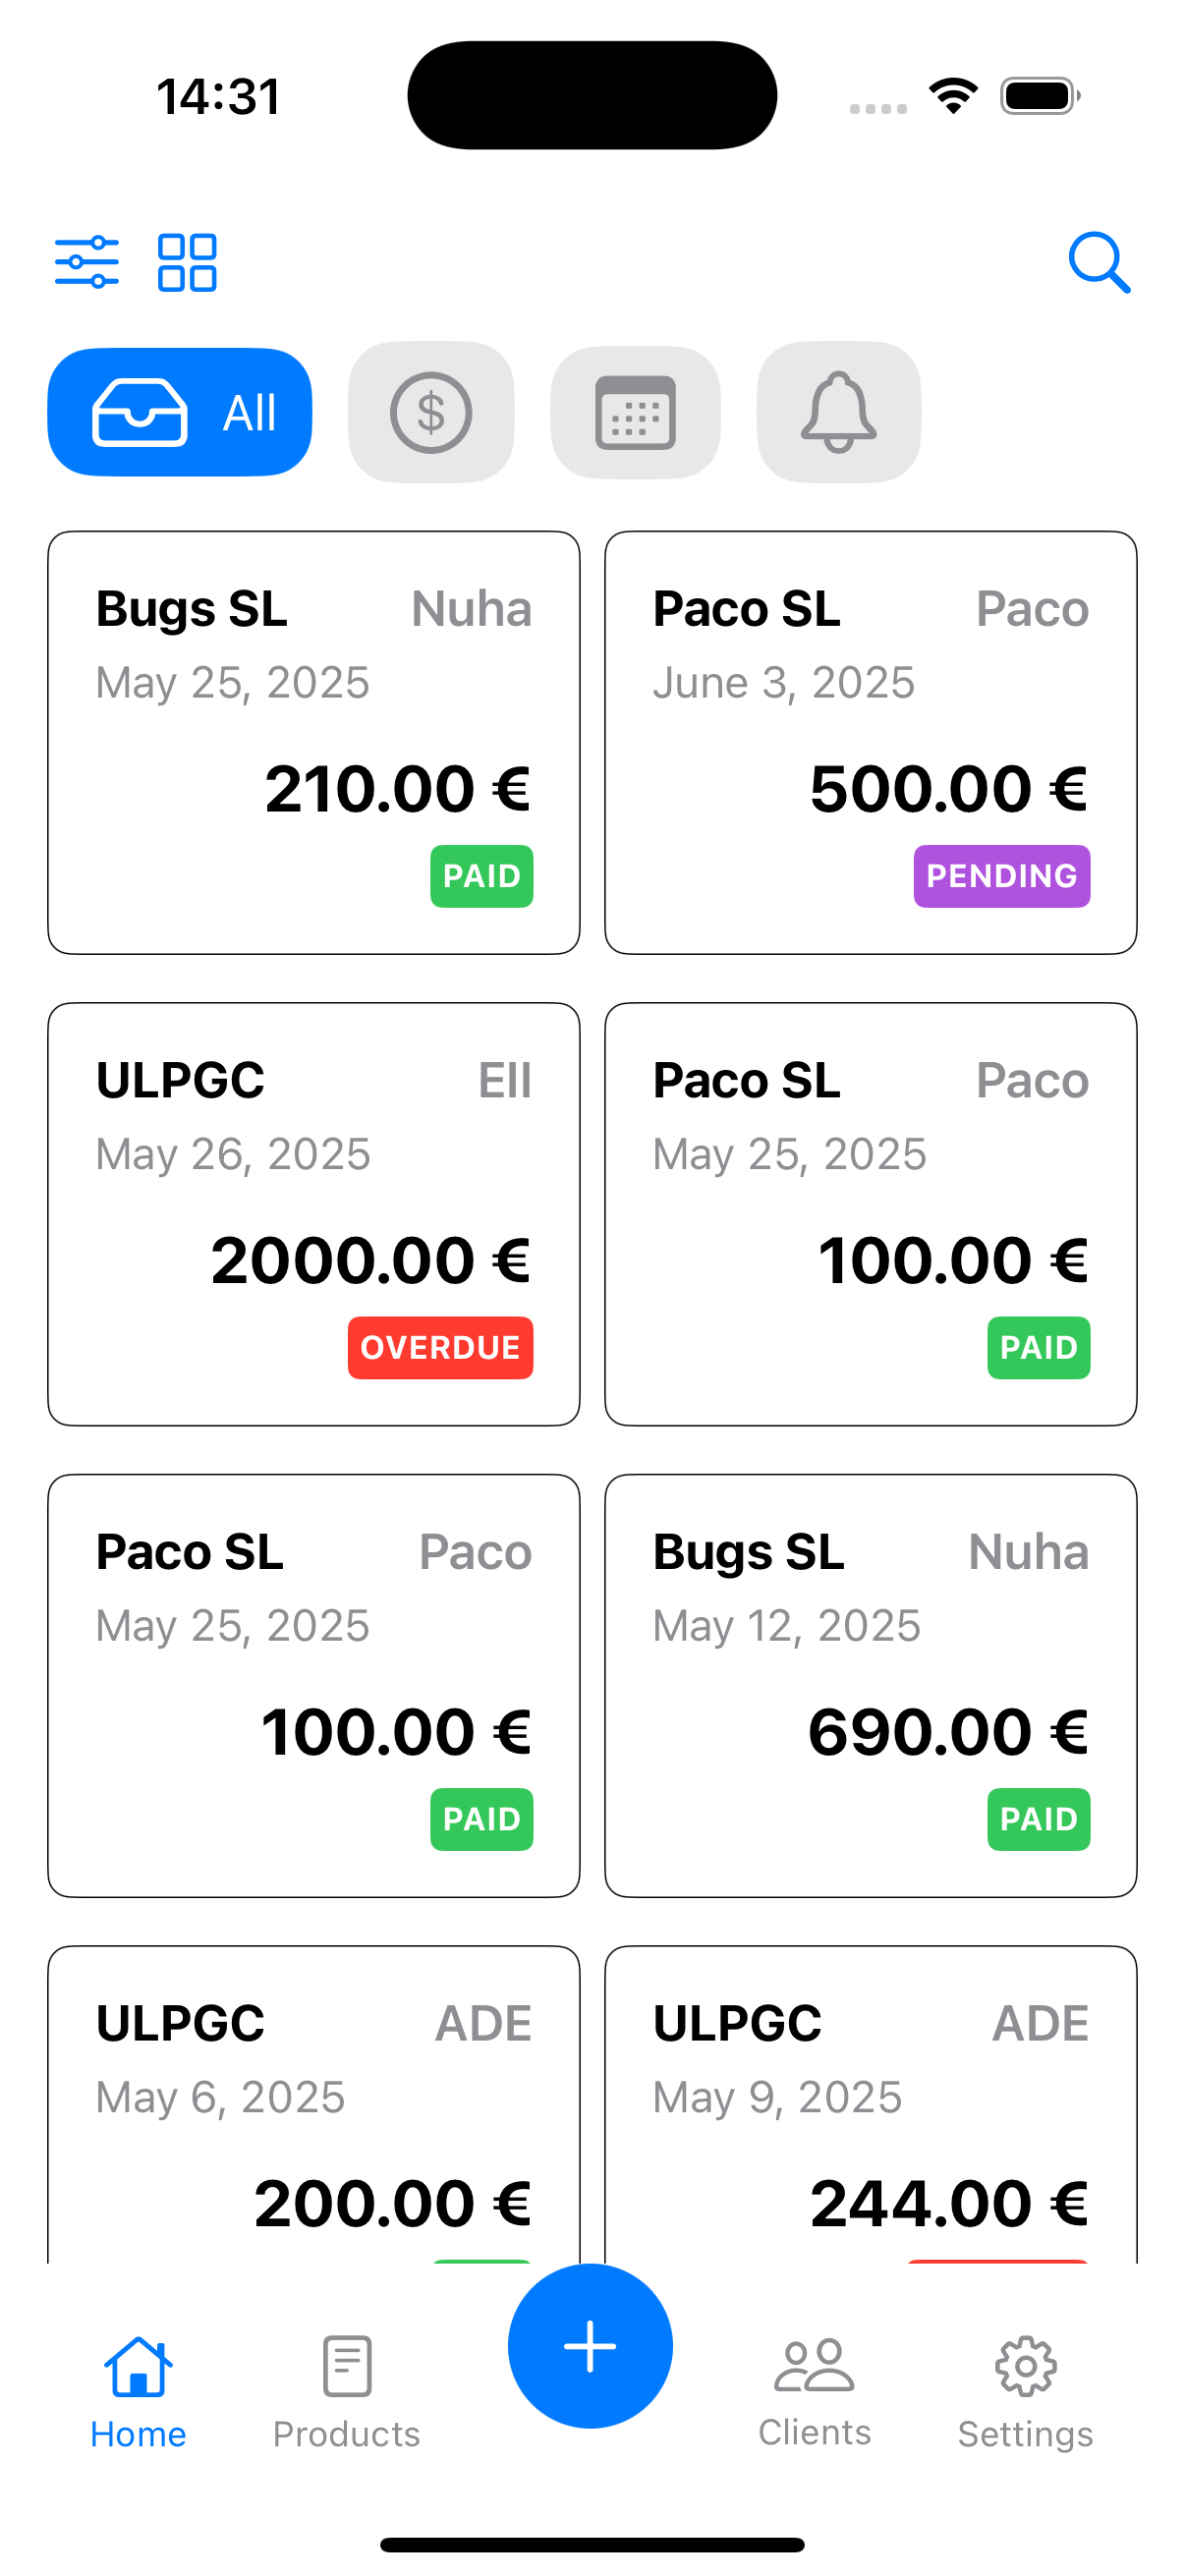
\includegraphics[width=0.8\textwidth]{Ilustraciones/ios_homeview.png}
    \caption{Vista principal con lista de facturas}
    \label{fig:home_view}
  \end{minipage}
\end{figure}

\begin{figure}[H]
	\centering
	%------------- Fila 2 -------------
  \begin{minipage}[t]{0.45\textwidth}
    \centering
    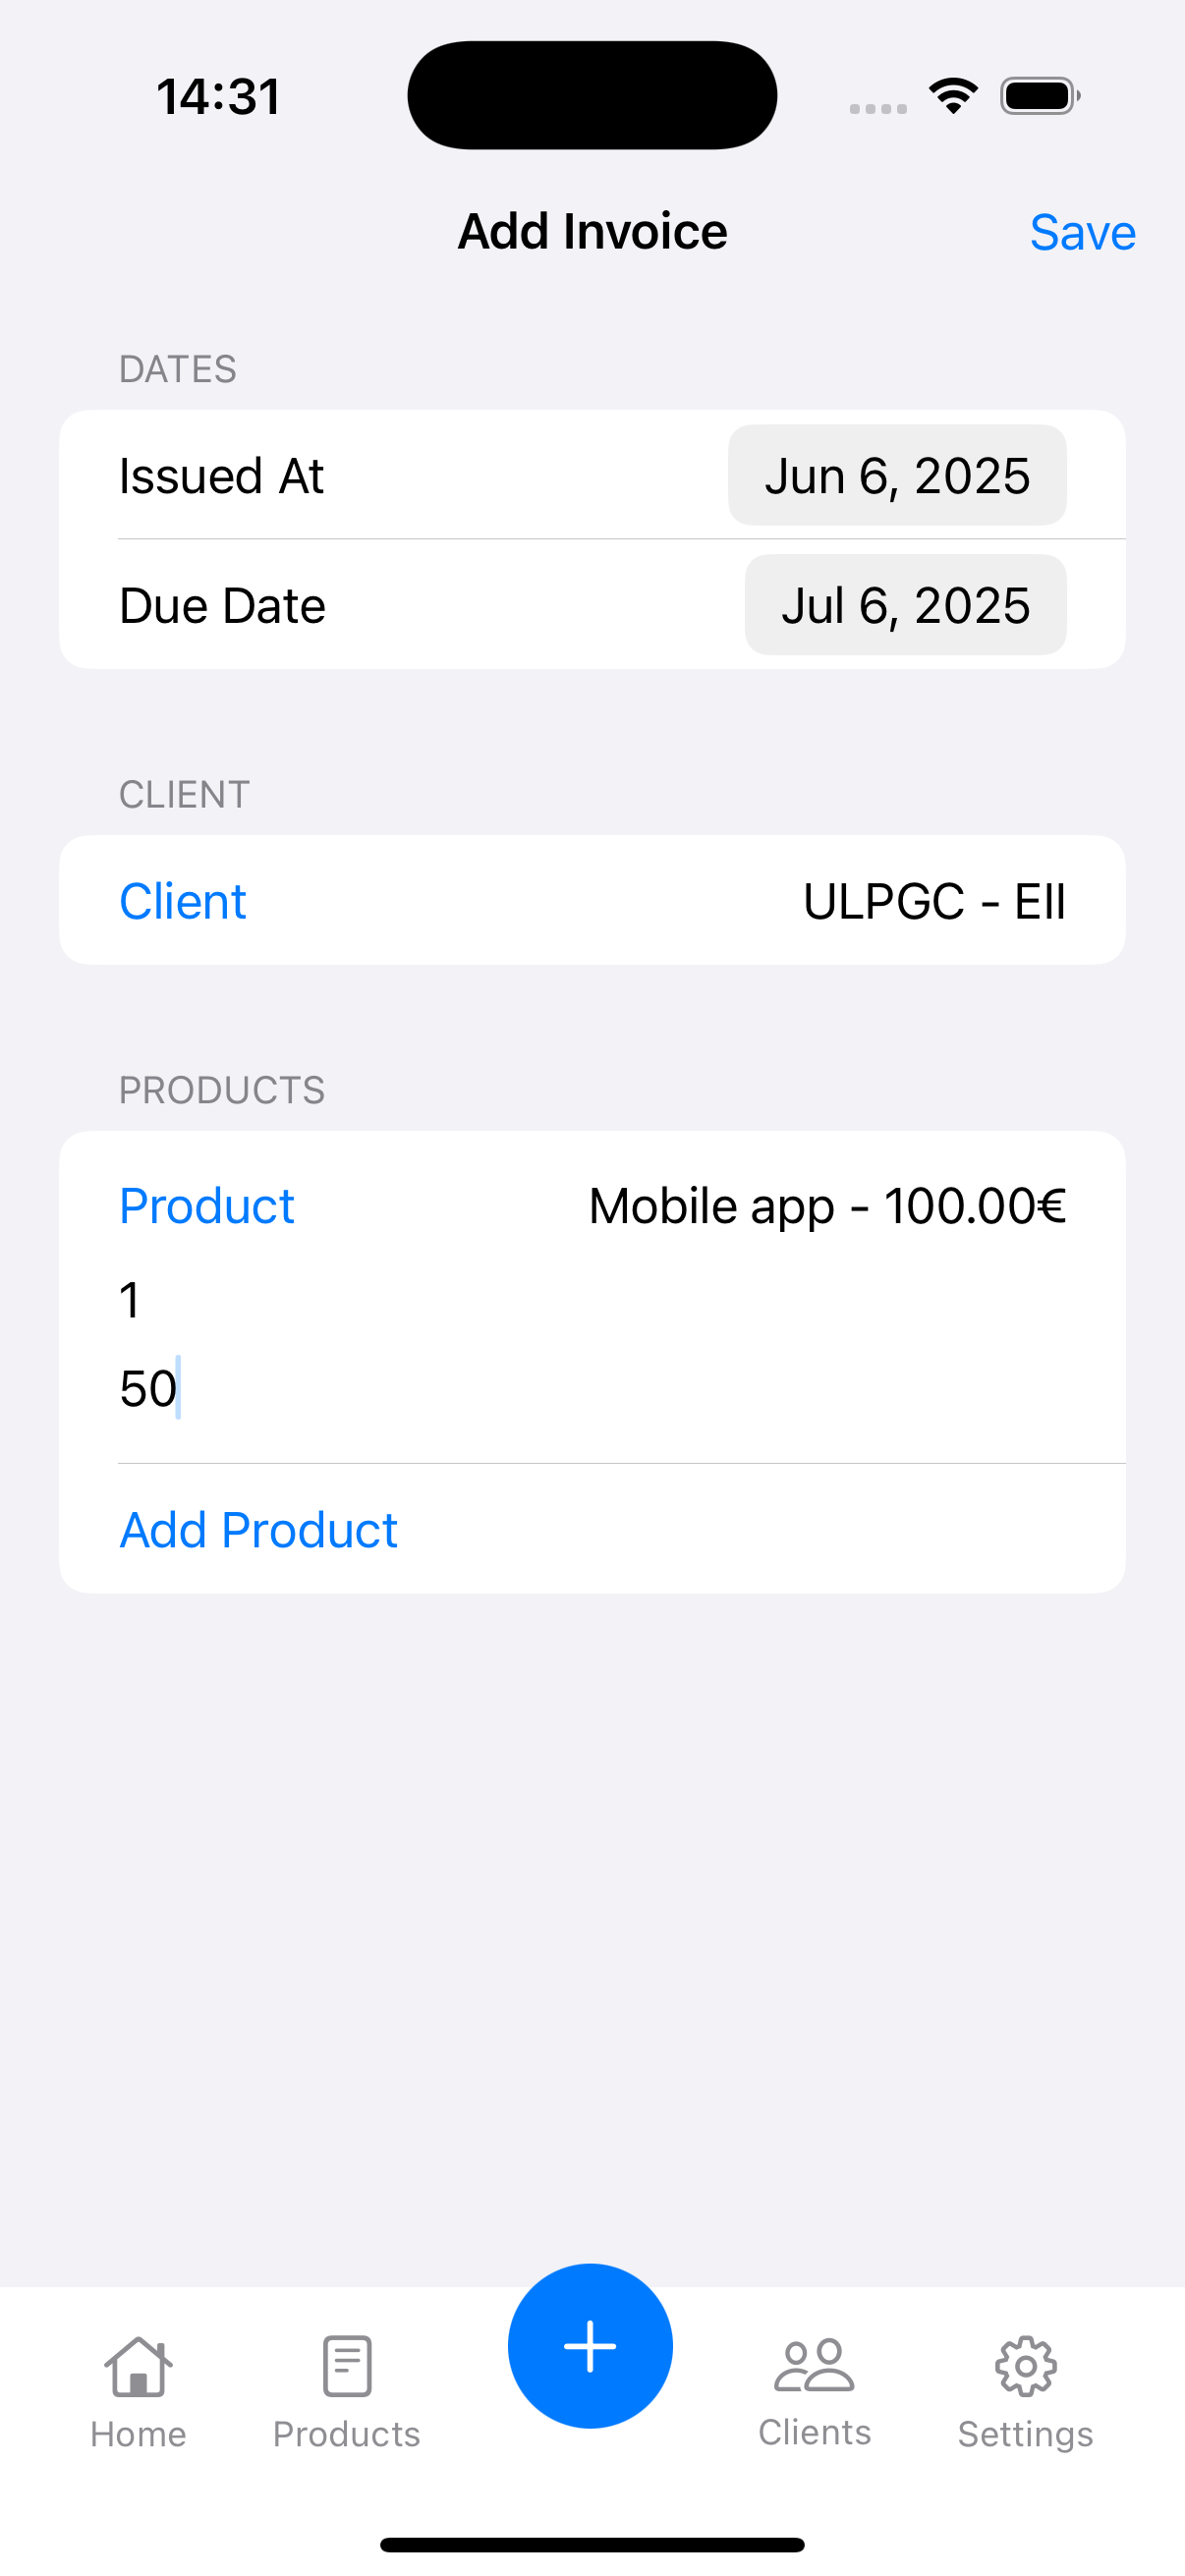
\includegraphics[width=0.8\textwidth]{Ilustraciones/ios_addinvoice.png}
    \caption{Formulario para añadir una nueva factura}
    \label{fig:add_invoice}
  \end{minipage}\hfill
  \begin{minipage}[t]{0.45\textwidth}
    \centering
    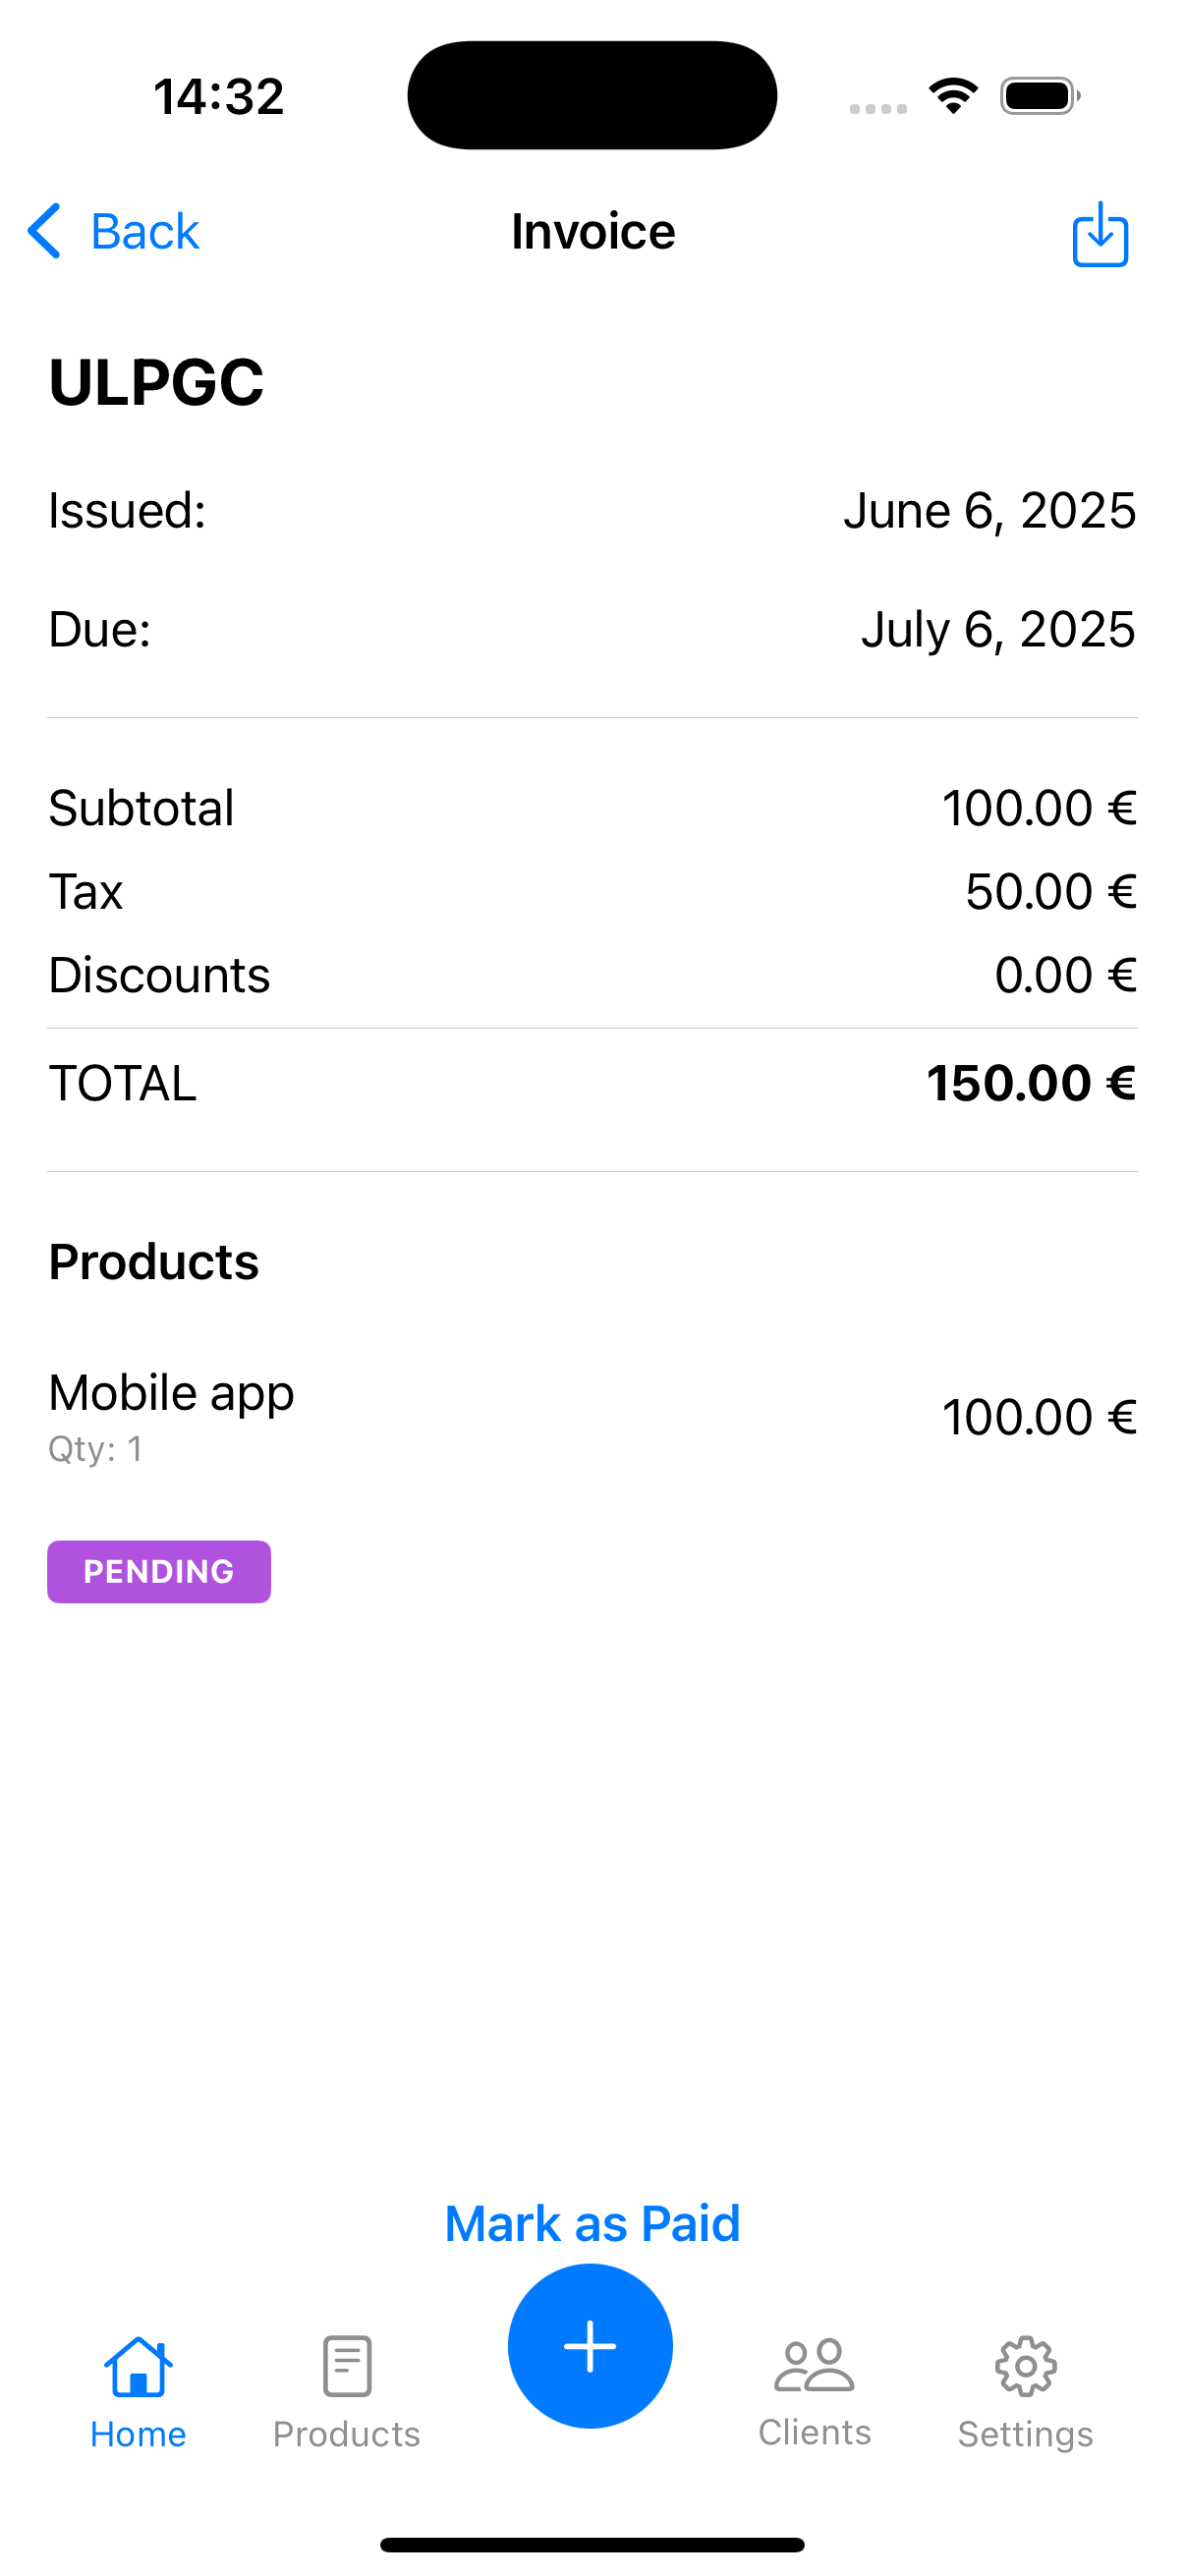
\includegraphics[width=0.8\textwidth]{Ilustraciones/ios_invoicedetails.png}
    \caption{Detalles de una factura con opción de generar PDF}
    \label{fig:invoice_details}
  \end{minipage}
\end{figure}

\begin{figure}[H]
	\centering
	%------------- Fila 3 -------------
  \begin{minipage}[t]{0.45\textwidth}
    \centering
    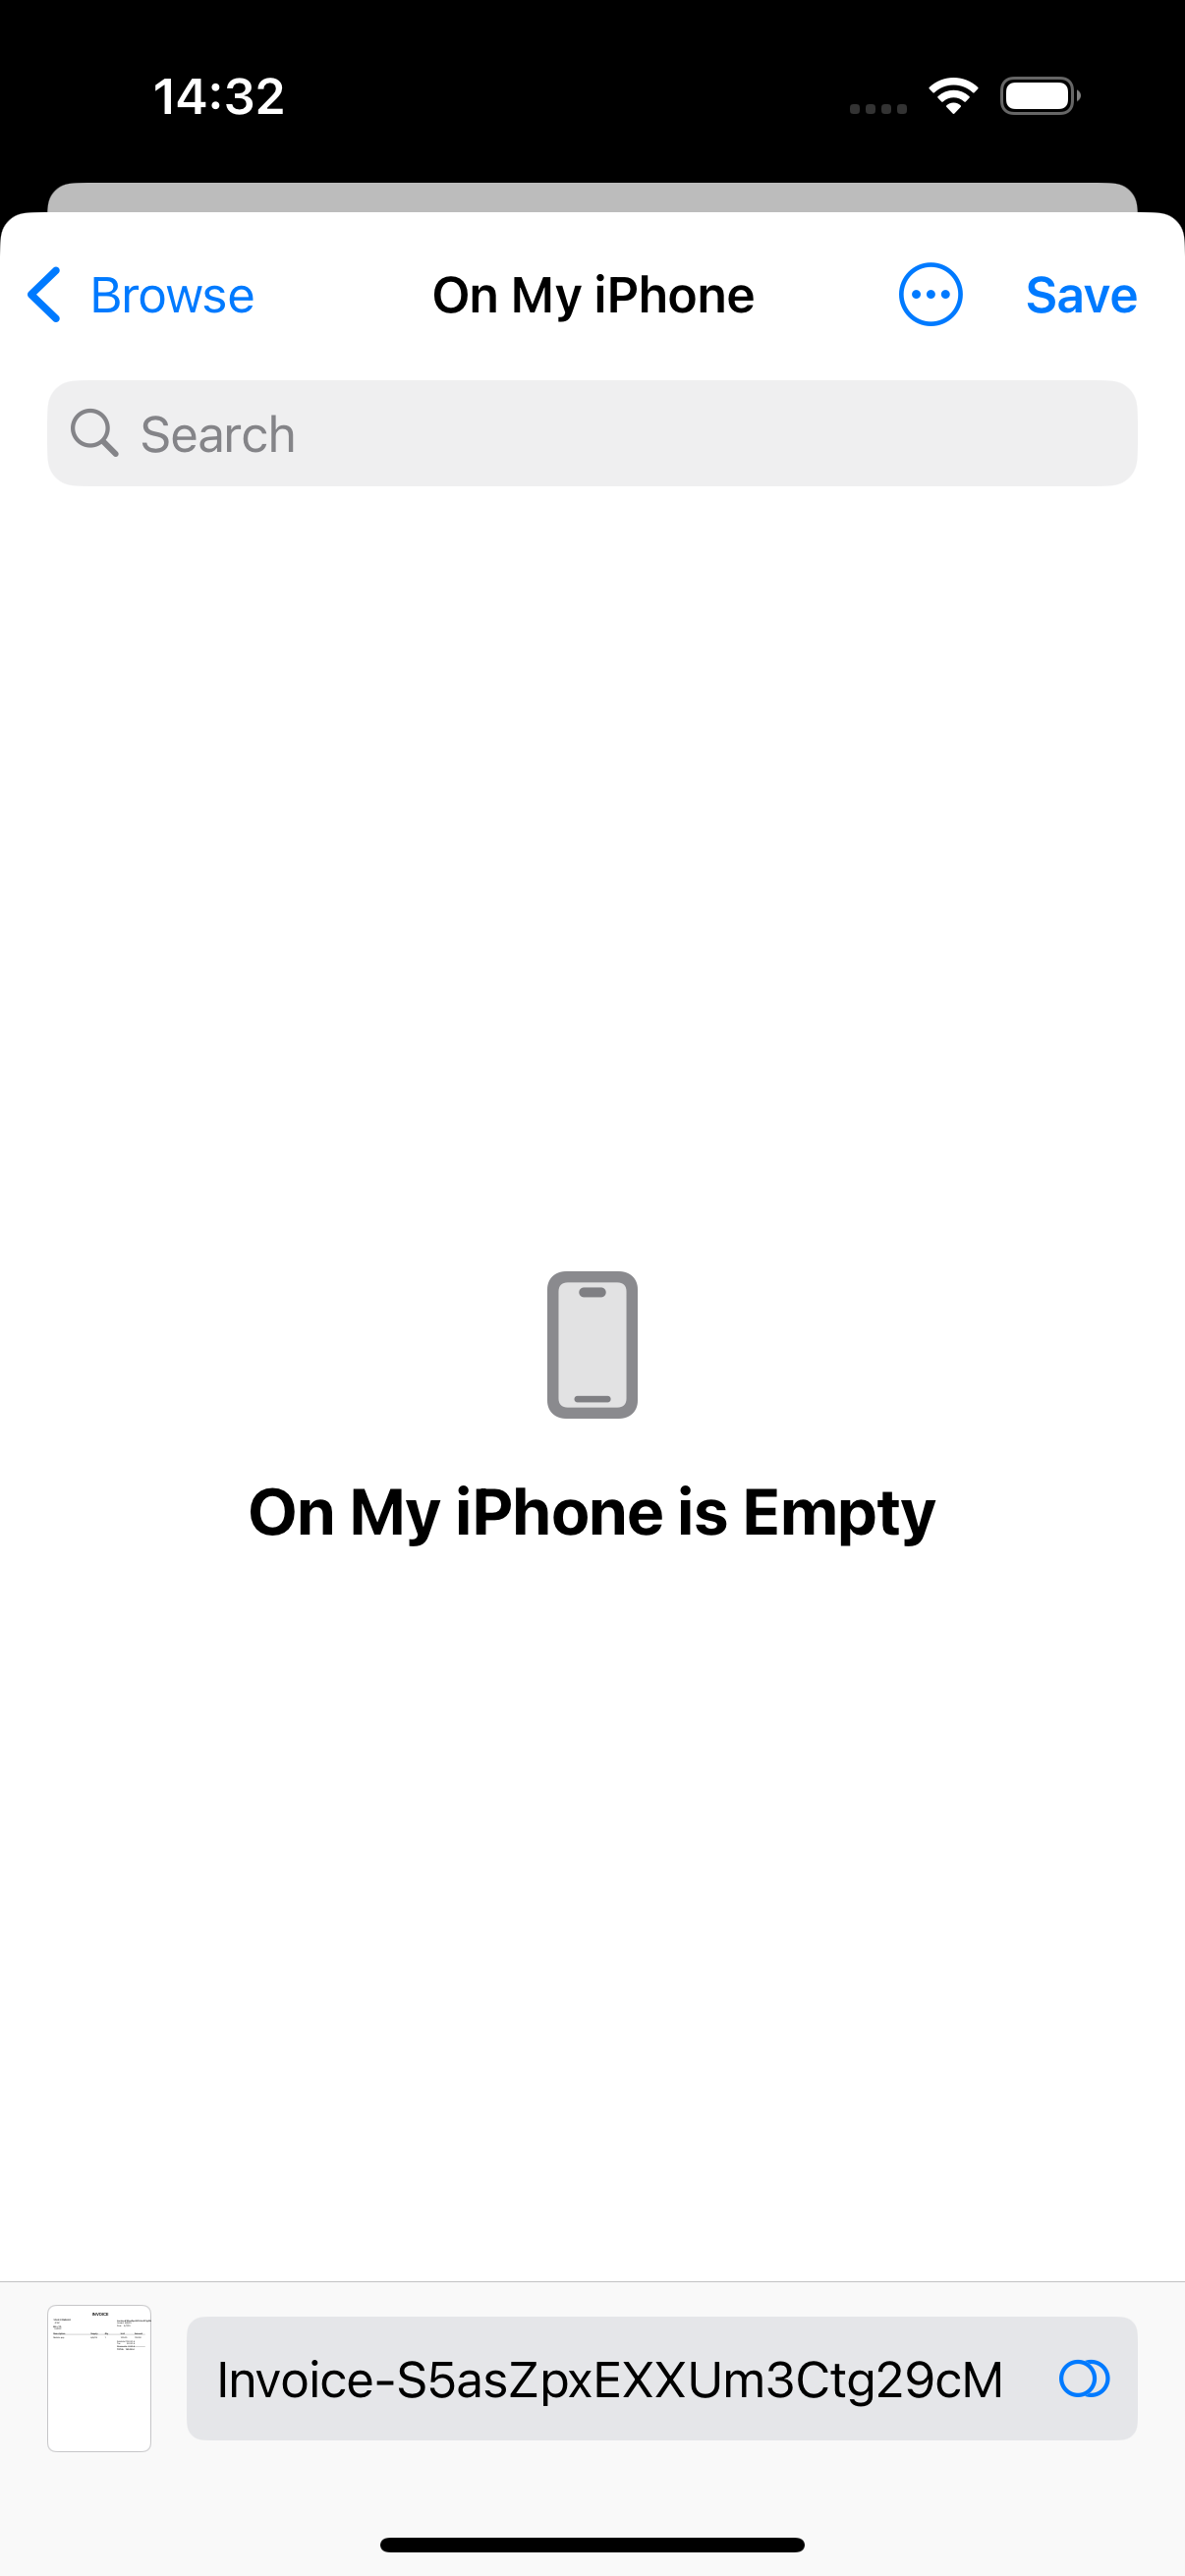
\includegraphics[width=0.8\textwidth]{Ilustraciones/ios_save_pdf.png}
    \caption{Generación del PDF de la factura}
    \label{fig:save_pdf}
  \end{minipage}
\end{figure}

\end{large}

%----------------------------------------------------------
\section{Implementación web}
%----------------------------------------------------------

\begin{large}

La parte web, aunque más ligera, ofrece tres funcionalidades clave: gráfica de pagos mensuales, listado de morosos y tabla con todas las facturas. A continuación se describe su estructura y lógica:

\end{large}

\subsection{Estructura general del proyecto}

\begin{large}

El repositorio para el portal web sigue la convención estándar de Astro:

\begin{figure}[H]
\centering
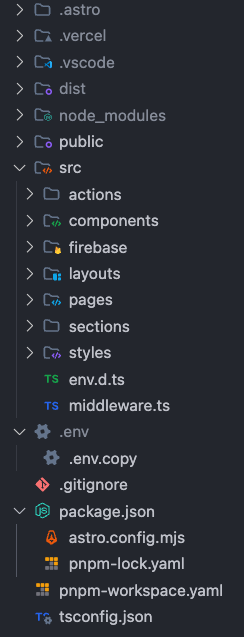
\includegraphics[width=0.3\textwidth]{Ilustraciones/astro_project_structure.png}
\caption{Estructura del proyecto Astro}
\label{fig:astro_project_structure}
\end{figure}

\begin{itemize}
  \item \textit{/src/pages}:
    \begin{itemize}
      \item \textit{index.astro}: página principal que importa los tres componentes.
      \item \textit{login.astro}: página de inicio de sesión para acceder al portal.
    \end{itemize}
  \item \textit{/src/components}:
    \begin{itemize}
      \item \textit{MoneyChart.astro}: renderiza la gráfica de barras usando \emph{lightweight-charts}.
      \item \textit{OverdueList.astro}: muestra tarjetas con clientes morosos y sus importes totales.
      \item \textit{InvoiceTable.astro}: tabla con todas las facturas (cliente, fecha, importe, estado) con ZingGrid.
			\item \textit{Header.astro}: barra de navegación con enlaces a las diferentes secciones y un botón de cierre de sesión.
			\item \textit{ButtonToScrollTop.astro}: botón que permite volver al inicio de la página.
    \end{itemize}
  \item \textit{/src/firebase}:
    \begin{itemize}
      \item \textit{firebase.ts}: inicializa Firebase con la configuración y exporta funciones e instancias de \textit{firestore} y \textit{auth}.
      \item \textit{config.ts}: carga la configuración desde el archivo \textit{.env} y exporta las variables necesarias.
    \end{itemize}
\end{itemize}

\end{large}

\subsection{Carga de datos y renderizado}

\begin{large}

Para cargar los datos de Firestore, se implementaron funciones asíncronas que se invocan en cada componente. A continuación se muestra cómo se obtienen todos los datos relevantes de un usuario a partir de su ID, que es el punto de partida para poblar las tablas y gráficas.

\begin{lstlisting}[language={}, caption={Función para obtener todos los datos de un usuario a partir de su ID}]
async function getAllDataForUser(userId: string) {
	const allData: any = {}

	// 1. get all businesses
	const businessesQuery = await query(collection(firestore, 'businesses'))
	const businessesSnapshot = await getDocs(businessesQuery)
	if (businessesSnapshot.empty) {
		console.log('No businesses found.')
		return []
	}

	// 2. filter all businesses where the user is in the employees collection
	const businesData = businessesSnapshot.docs.map(async (doc) => {
		const businessData = doc.data()
		const businesId = doc.id
		const employees = await getEmployeesBy(businesId)
		const isEmployee =
			employees.filter((employee: any) => employee.userId === userId) || null
		if (!isEmployee || isEmployee.length === 0) {
			return null
		}
		return {
			id: businesId,
			...businessData,
		}
	})
	const businesses = (await Promise.all(businesData)).filter((b) => b !== null)
	if (businesses.length === 0) {
		console.log('No businesses found for this user.')
		return []
	}
	const businessId = businesses[0].id
	allData.businesses = businesses

	// 3. get all invoices that are inside the business collection
	const invoices = getInvoicesBy(businessId)
	allData.invoices = await invoices

	// 4. get all clients that are inside the business collection
	const clients = getClientsBy(businessId)
	allData.clients = await clients

	// 5. get all products that are inside the business collection
	const products = getProductsBy(businessId)
	allData.products = await products

	// 6. get all employees that are inside the business collection
	const employees = getEmployeesBy(businessId)
	allData.employees = await employees

	return allData
}
\end{lstlisting}

Una vez se retorna el objeto \textit{allData}, cada componente puede acceder a los datos necesarios del objeto, el cual se actualizará automáticamente cuando cambien los datos en Firestore.

\begin{lstlisting}[language={}, basicstyle=\ttfamily\small, caption={Función para listar todas las facturas en la tabla}]
function listAllInvoices(allData: any) {
    const invoiceGrid = document.querySelector('#invoiceGrid') as any
    if (!invoiceGrid) return
    const invoiceGridData = allData.invoices.map((invoice: any) => {
        const client = allData.clients.find(
            (client: any) => client.id === invoice.clientId
        )
        return {
            client: client.companyName,
            issued: new Date(invoice.issuedAt.seconds * 1000)
              .toLocaleDateString(
                'es',
                {
                    day: '2-digit',
                    month: '2-digit',
                    year: 'numeric',
                }
            ),
            total: `${invoice.totalAmount}${invoice.currency}`,
            status: invoice.status,
        }
    })
    invoiceGrid.data = invoiceGridData
}
\end{lstlisting}

Para el listado de morosos, \textit{OverdueList.astro} filtra facturas cuyo estado sea “Overdue” y las agrupa por cliente.

\begin{lstlisting}[language={}, basicstyle=\ttfamily\small, caption={Función para listar clientes morosos}]
function listOverdueClients(allData: any) {
	const overdueCards = document.querySelector('#overdueClientsCards')

	let dictOverdueClients: any = {}

	allData.clients.forEach((client: any) => {
		dictOverdueClients[client.id] = {
			name: client.companyName,
			amount: 0,
			currency: '',
		}
	})

	allData.invoices.forEach((invoice: any) => {
		if (invoice.status === 'Overdue') {
			const client = dictOverdueClients[invoice.clientId]
			if (client) {
				client.amount += invoice.totalAmount
				client.currency = invoice.currency
			}
		}
	})
    
	/* Inyectar HTML */
}
\end{lstlisting}

\end{large}

\subsection{Librerías externas}

\begin{large}

Para el portal web se utilizaron varias librerías externas que facilitan la creación de gráficos, tablas y la experiencia de usuario:

\begin{itemize}
\item \textbf{lightweight-charts}: Permite renderizar gráficas de barras y líneas de forma eficiente y responsiva\,\cite{lightweight_charts}. Se emplea en el componente \textit{MoneyChart.astro} para mostrar la evolución mensual de los pagos.
\item \textbf{ZingGrid}: Framework para crear tablas interactivas y personalizables\,\cite{zinggrid}. Se utiliza en \textit{InvoiceTable.astro} para listar todas las facturas con ordenación, filtrado y paginación.
\end{itemize}

Estas librerías permiten construir una interfaz moderna y dinámica, reduciendo el esfuerzo de desarrollo y mejorando la experiencia del usuario final.

\end{large}

\subsection{Despliegue del portal en Vercel}

\begin{large}
	
El portal web se despliega en Vercel siguiendo el flujo de integración continua:

\begin{enumerate}
  \item Cada vez que se hace \emph{push} a la rama \textit{main}, Vercel detecta el cambio y ejecuta el comando \textit{pnpm run build}.
  \item Una vez compilado, Vercel optimiza los activos estáticos y publica el sitio en una URL de producción.
\end{enumerate}

A continuación se muestra una captura del panel de Vercel donde se observa el estado del último despliegue y la URL asignada.

\begin{figure}[H]
\centering
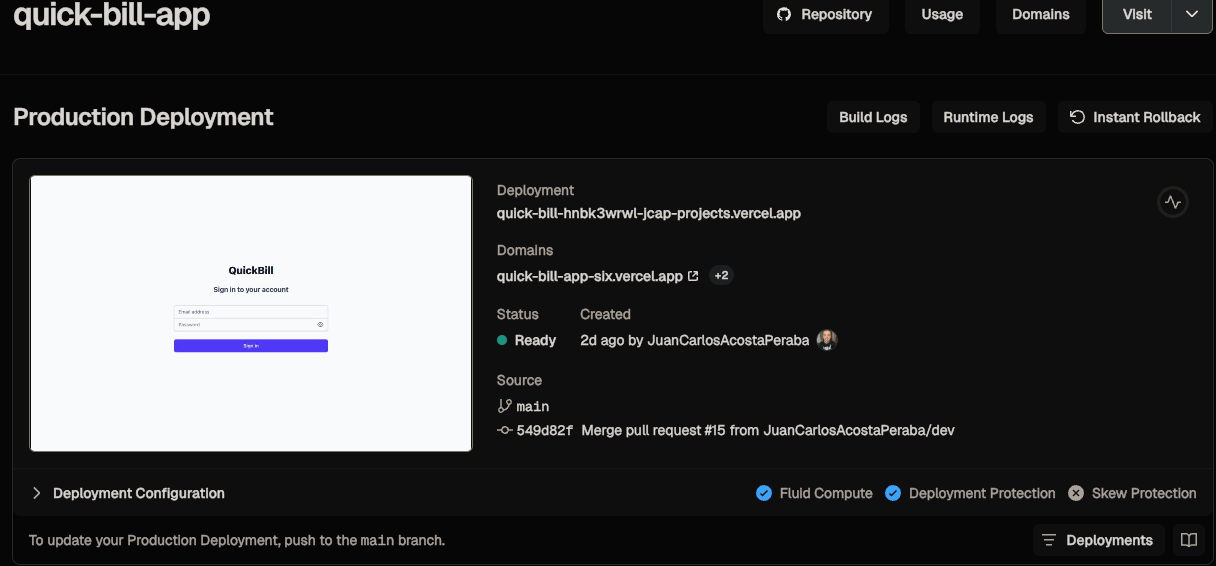
\includegraphics[width=0.8\textwidth]{Ilustraciones/vercel_deploy.png}
\caption{Panel de Vercel con el estado del último despliegue}
\label{fig:vercel_deploy}
\end{figure}

\begin{figure}[H]
\centering
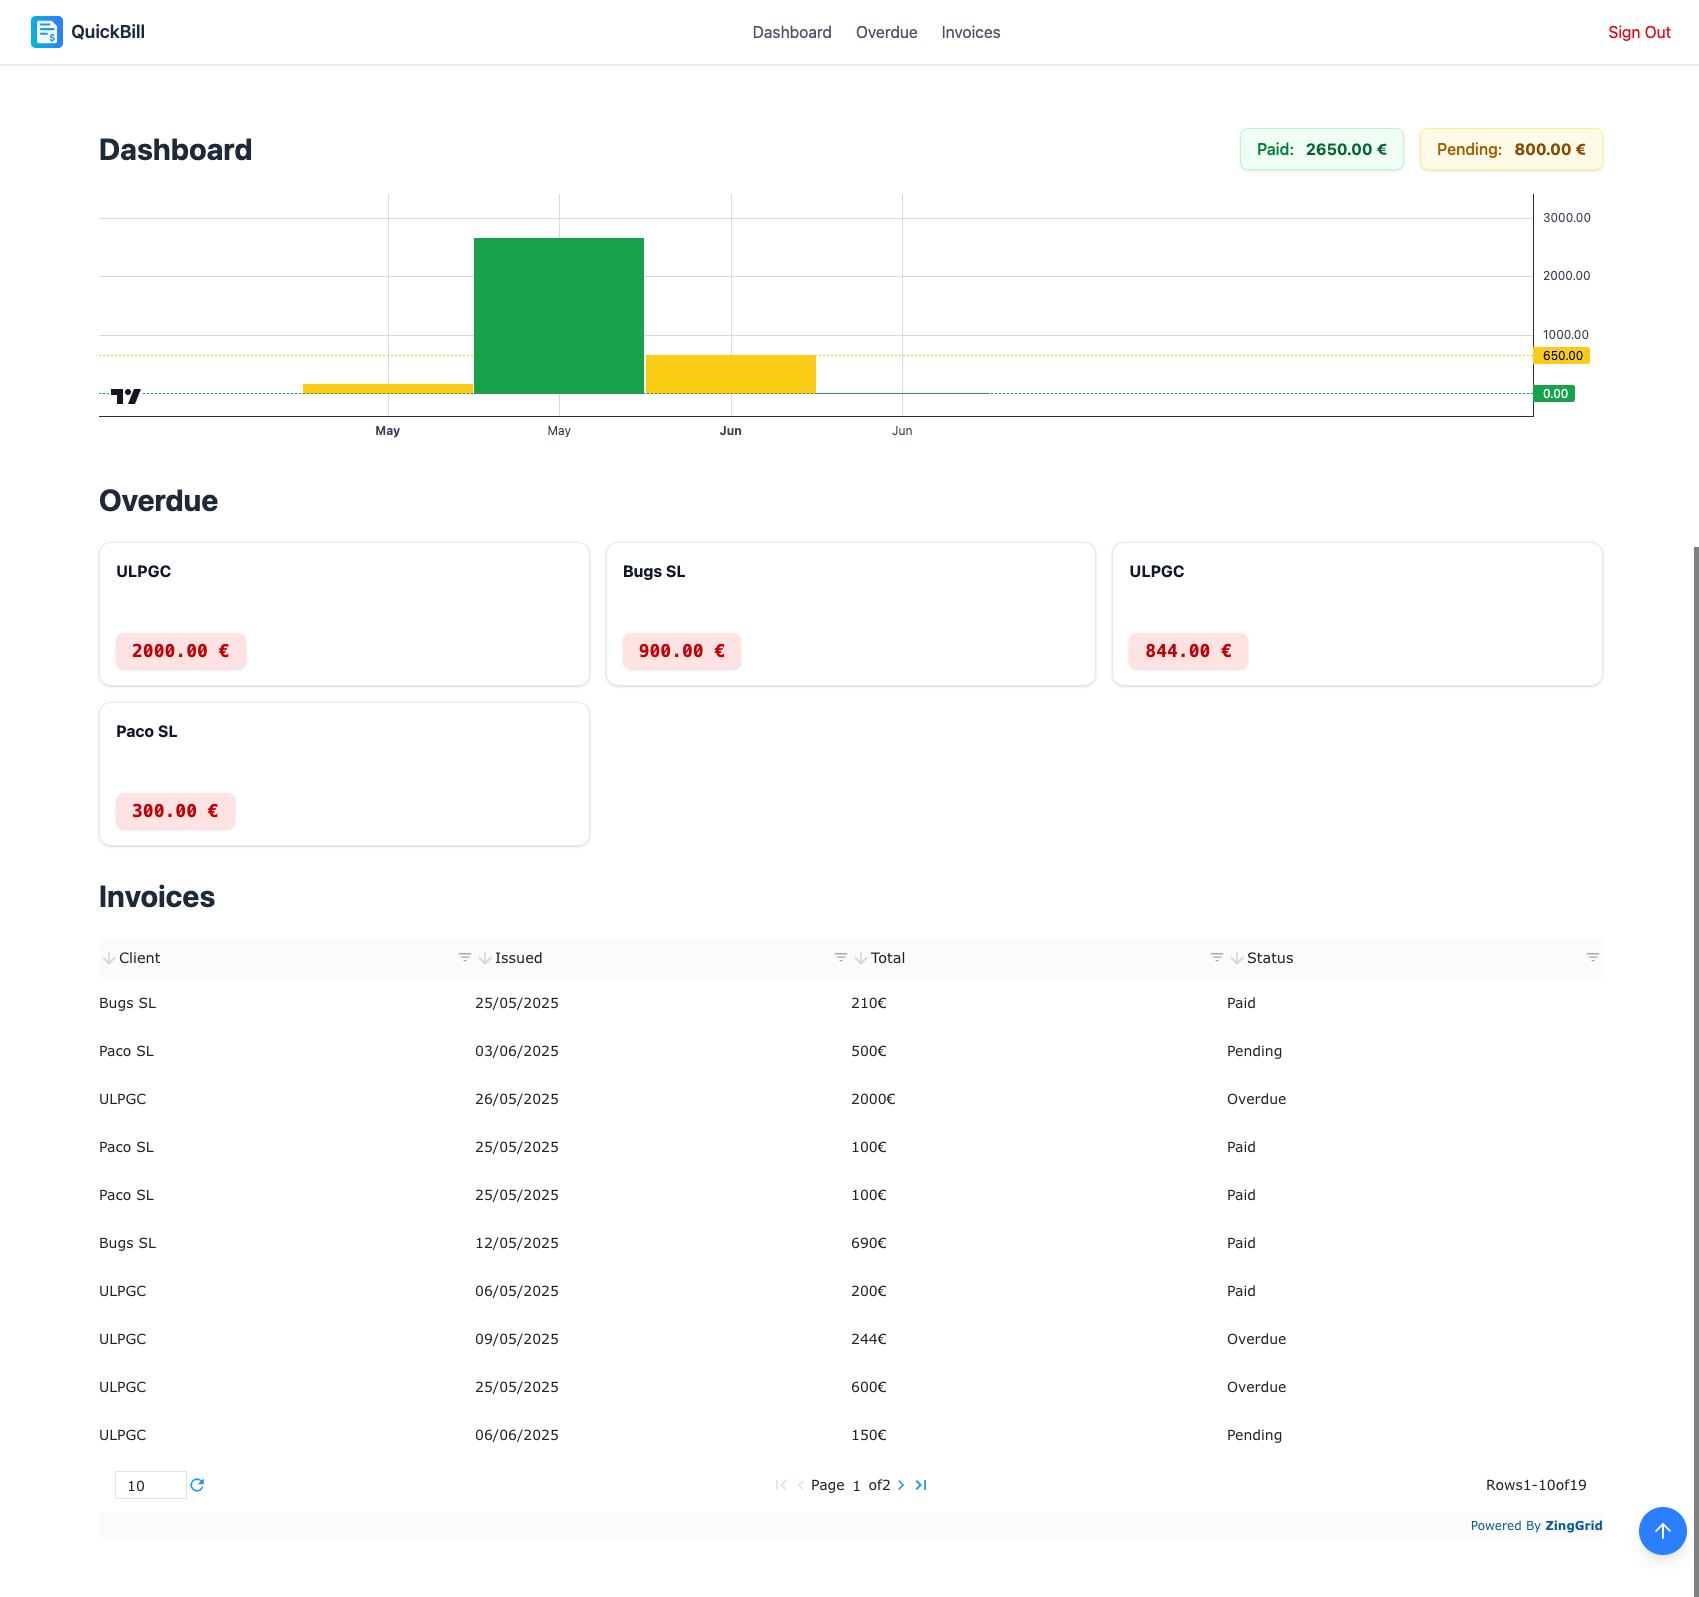
\includegraphics[width=0.8\textwidth]{Ilustraciones/vercel_deployed.png}
\caption{Portal web desplegado en Vercel}
\label{fig:vercel_deployed}
\end{figure}

\noindent El portal web está disponible en la URL \url{https://quick-bill-app-six.vercel.app/}, donde los usuarios pueden iniciar sesión y acceder a las funcionalidades descritas. Algunas cuentas de prueba que se pueden usar son:
\begin{itemize}
	\item \texttt{jcacostaperaba98@gmail.com} / \texttt{qwerty123456}
	\item \texttt{juancarlos@jcap.com} / \texttt{estoEsUnT3st}
\end{itemize}

\end{large}
